\section{Aufgabenstellung und Versuch}

Aus den bereits aufgestellten DGL-System kann das Blockschaltbild in Simulink
erstellt werden.

\begin{figure}[H]
    \centering
    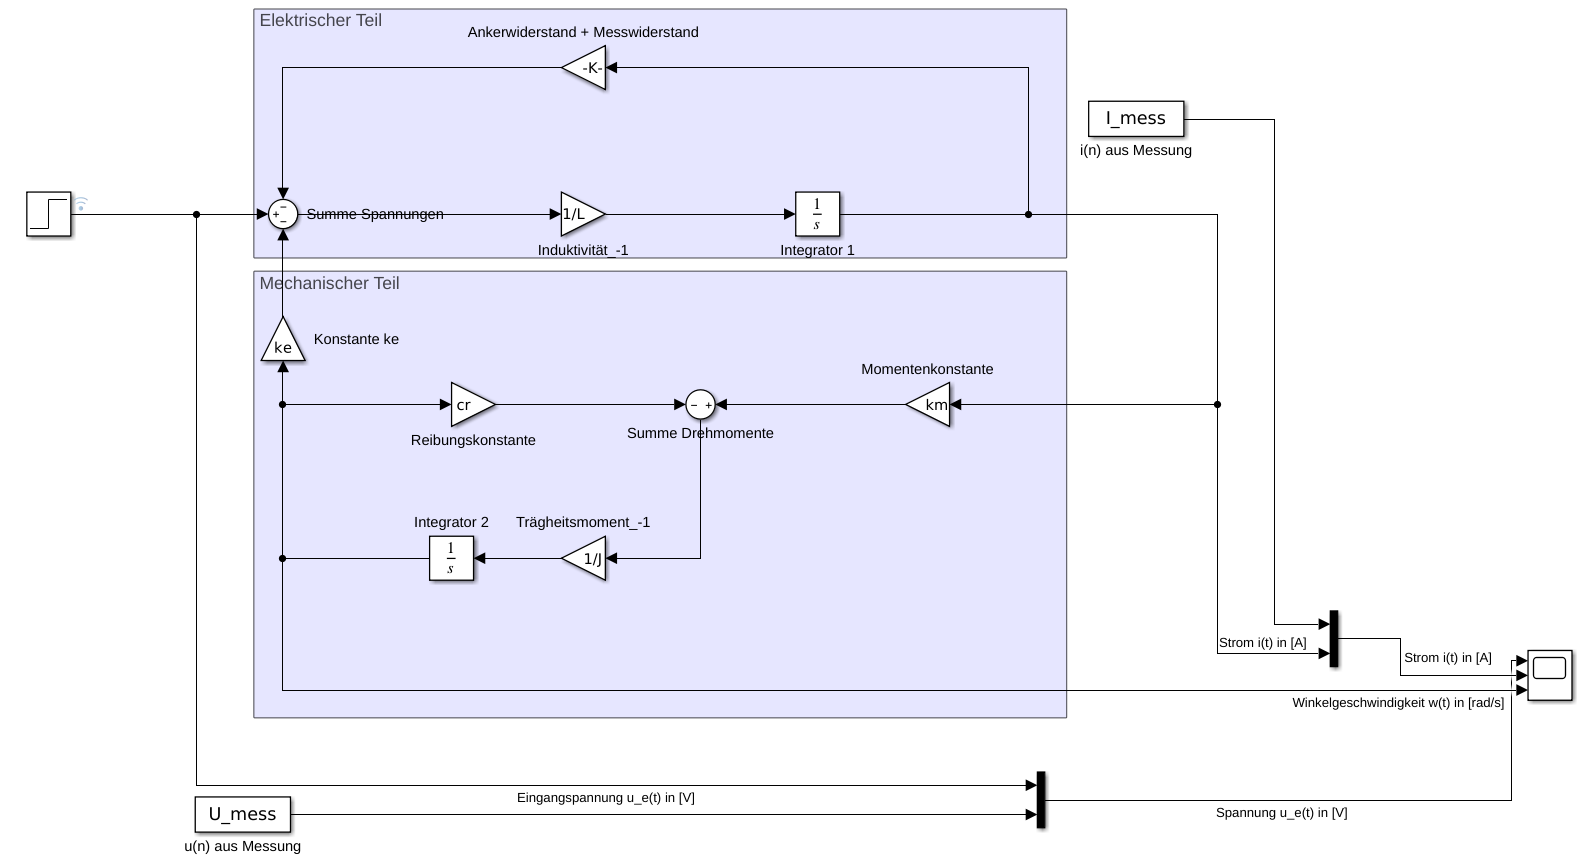
\includegraphics[width=1\textwidth]{sl_modell.png}
    \caption{Blockschaltbild in Simulink}
    \label{fig:Blockschaltbild}
\end{figure}

Als Eingang wurde ein Step-Block benutzt und als Ausgang Scope-Block.
Die erste DGL wurden im oberen Teil des Modell realisiert und beschreibt
den elektrischen Teil des Systems. Im unteren wird der mechanische Teil
des Motors modelliert der aus der zweiten DGL hervorgeht.

